\chapter{Implementation}
[Text here]

\section{Hardware implementation}
[Text here]

\subsection{Printed Circuit Boards}

Our design additionally consists of two Printed Circuit Boards (PCBs), one for each used microcontroller. The first PCB designed is for the PIC18F slave microcontroller. It contains connections for the solenoid, and its control circuit which consists of an optocoupler and a Darlington NPN bipolar transistor (TIP120). It also contains connections for the servo motor and its control circuit which is a simple MOSFET transistor circuit.  The board also contains connections for the NRF24 module.

\begin{figure}[h]
	\centering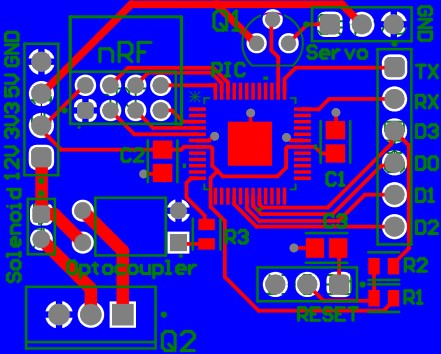
\includegraphics[height=5cm]{./images/picpcb}
	\caption{PIC18F PCB Design}
\end{figure}

The second designed PCB is for the ESP32 master controller. This PCB consists of headers for the ESP32 controller itself, and headers for each of the DRV8825 modules. It has a switch for on board adjustment of the drivers' control pins. It also contains connections for the NRF24 module.

\begin{figure}[h]
	\centering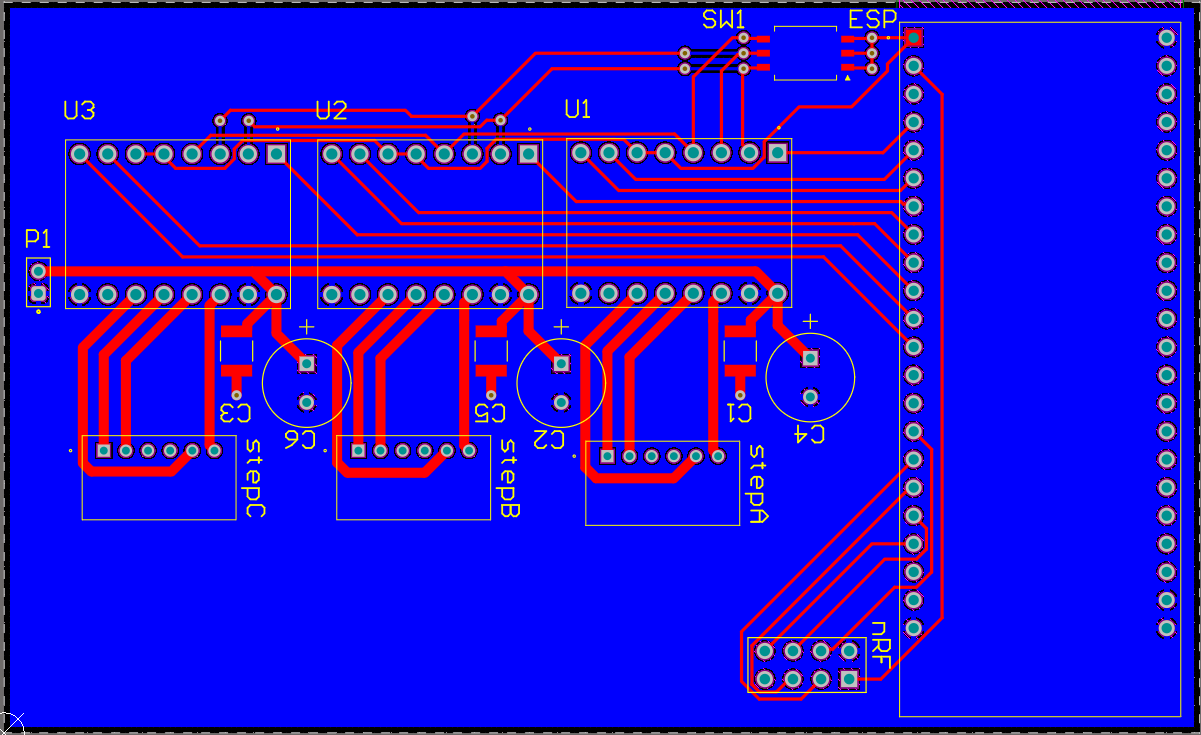
\includegraphics[height=5cm]{./images/esppcb}
	\caption{ESP32 PCB Design}
\end{figure}


\section{Software implementation}

[TEXT]
